\section{Admitere F iulie 2024}

2024.A.1. La o sursă de tensiune ideală se conectează 15 ampermetre ideale, fiecare conectat în serie cu câte un rezistor cu rezistența $R_{i}(i=1, \ldots, 15)$ și 15 voltmetre ideale, fiecare dintre ele fiind conectat în paralel cu câte un rezistor cu rezistența $R$, ca în figură. Voltmetrul $V_{1}$ indică $U_{1}=9 \mathrm{~V}$, iar primele două ampermetre indică $I_{1}=2,9 \mathrm{~mA}$ și $I_{2}=2,6 \mathrm{~mA}$. Suma valorilor indicate de celelalte voltmetre este: (9 pct.)\\ a) $7,8 \mathrm{~V}$; b) $80 \mathrm{~V}$; c) $9 \mathrm{~V}$; d) $90 \mathrm{~V}$; e) $8 \mathrm{~V}$; f) $78 \mathrm{~V}$.\\ 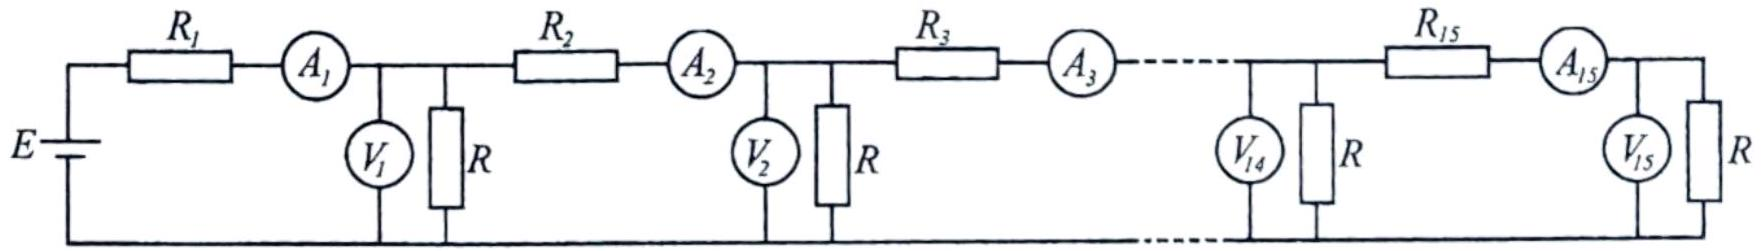
\includegraphics[width=0.4\linewidth]{images/2025_08_29_f6247b646b21fa124082g-1(1)}\\ Considerăm figura problemei:\\ \begin{center} 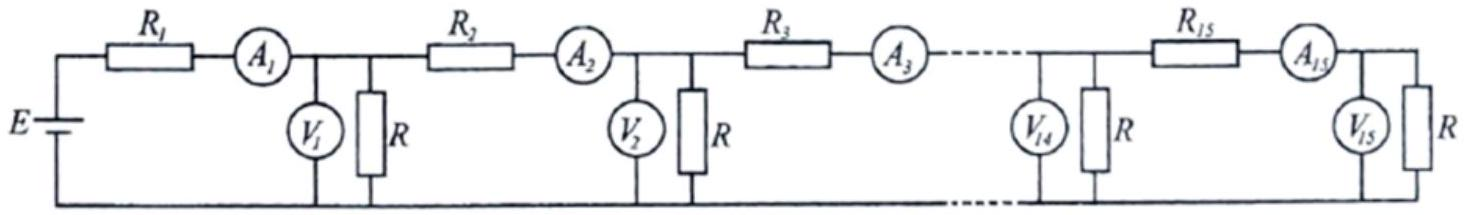
\includegraphics[width=0.4\linewidth]{images/2025_08_29_e254769008c62e16ba92g-1} \end{center}\\ Avem:\\ $\sum_{i=2}^{15} U_{i}=r \sum_{i=2}^{15} i \\ \sum_{i=2}^{15} i=\left(I_{2}-I_{3}\right)+\left(I_{3}-I_{4}\right)+\cdots+\left(I_{13}-I_{14}\right)+\left(I_{14}-I_{15}\right)=I_{2} \\ \sum U_{i}=r \cdot I_{2} \\ i_{1}=I_{1}-I_{2} \\ U_{i}=i_{1} \cdot r \Rightarrow R=\frac{U_{i}}{I_{1}-I_{2}}=\frac{9}{2,9-2,6}=\frac{9}{0,3}=30 \Omega \Rightarrow \sum_{i=2}^{15} U_{i}=30 \cdot 2,6=78 \mathrm{~V}$. Răspuns corect f.\\

2024.A.2. Se consideră circuitul din figură în care sursa de tensiune este ideală. Raportul $I_{1} / I_{2}$ dintre curentul $I_{1}$ indicat de ampermetru când întrerupătorul $K$ este închis și curentul $I_{2}$ indicat de ampermetru când întrerupătorul $K$ este deschis este: (9 pct.)\\ a) $\frac{3}{2}$; b) $\frac{3}{4}$; c) $\frac{9}{8}$; d) $\frac{8}{9}$; e) $1$; f) $\frac{4}{3}$.\\ 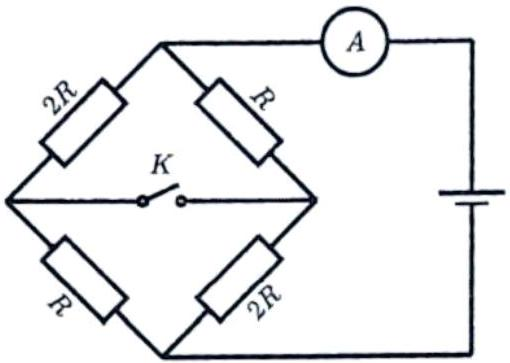
\includegraphics[width=0.4\linewidth]{images/2025_08_29_f6247b646b21fa124082g-1}\\ Considerăm figura problemei:\\ \begin{center} 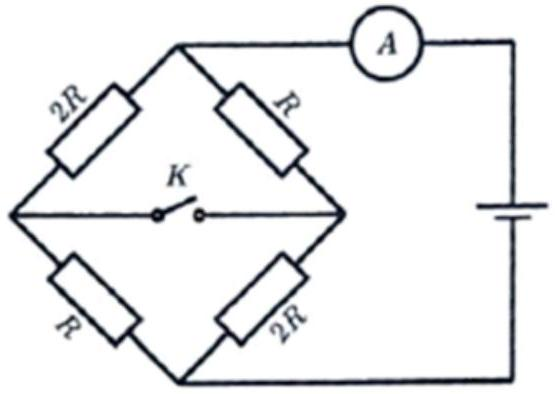
\includegraphics[width=0.4\linewidth]{images/2025_08_29_e254769008c62e16ba92g-1(1)} \end{center}\\ Cu $K$ închis: $\left(\frac{1}{R}+\frac{1}{2 R}\right)^{-1} \cdot 2=R_{e} \Rightarrow R_{e_{1}}=\frac{2 R}{3} \cdot 2=\frac{4 R}{3}$;\\ Cu $K$ deschis: $\left(\frac{2}{3 R}\right)^{-1}=R_{e} \Rightarrow R_{e_{2}}=\frac{3 R}{2}$;\\ Obținem: $I_{1} R_{e_{1}}=I_{2} R_{e_{2}} \Rightarrow \frac{I_{1}}{I_{2}}=\frac{R_{e e}}{R_{e_{1}}}=\frac{3 R}{2} \cdot \frac{3}{4 R}=\frac{9}{8}$. Răspuns corect c.\\

2024.A.3. Un mol de gaz ideal trece printr-o transformare în care relația între presiune și volum este $p=a\left[1-\frac{1}{2}\left(\frac{b}{V}\right)^{2}\right]$, unde $a=3,328 \cdot 10^{5} \mathrm{~Pa}$ și $b=1,6$ litri. Atunci când volumul $V$ al gazului variază de la $1,6$ litri la $3,2$ litri, temperatura gazului creşte cu ($R=8,32 \mathrm{~J} / \mathrm{mol} \cdot K$): (9 pct.)\\ a) $64 \mathrm{~K}$; b) $32 \mathrm{~K}$; c) $3200 \mathrm{~K}$; d) $80 \mathrm{~K}$; e) $320 \mathrm{~K}$; f) $3,2 \mathrm{~K}$.\\ Relația de bază a transformării este:\\ $p=a\left[1-\frac{1}{2}\left(\frac{b}{V}\right)^{2}\right]; \quad a=3,328 \cdot 10^{5} \mathrm{~Pa}; \quad b=1,6$ litri\\ Pentru cele două situații, avem:\\ $p_{1}=a\left[1-\frac{1}{2}\left(\frac{b}{b}\right)^{2}\right]=\frac{a}{2}$;\\ $p_{2}=a\left[1-\frac{1}{2}\left(\frac{b}{2 b}\right)^{2}\right]=a\left[1-\frac{1}{8}\right]=\frac{7 a}{8}$;\\ Scriem ecuațiile de stare pentru aceste situații:\\ $p_{1} V_{1}=\nu R T_{1} \Rightarrow \frac{a b}{2}=\nu R T_{1} \Rightarrow T_{1}=\frac{a b}{2 \nu R}$\\ $p_{2} V_{2}=\nu R T_{2} \Rightarrow \frac{7 a}{8} \cdot 2 b=\nu R T_{2} \Rightarrow \frac{7 a b}{4}=\nu R T_{2} \Rightarrow T_{2}=\frac{7 a b}{4 \nu R}$\\ Deci diferența de temperatură este:\\ $T_{2}-T_{1}=\frac{7 a b}{4 \nu R}-\frac{a b}{2 \nu R}=\frac{a b}{2 \nu R}(3,5-1)=\frac{3,328 \cdot 10^{5} \cdot 1,6 \cdot 10^{-3}}{2 \cdot 8,32}(2,5)=32 \cdot 2,5=80 \mathrm{~K}$. Răspuns corect d.\\

2024.A.4. Două mobile pornesc simultan din punctul $A$ de-a lungul laturilor unui circuit de forma unui triunghi dreptunghic $A B C$ deplasându-se cu viteze constante. Primul se îndreaptă spre punctul $C$ iar cel de-al doilea spre punctul $B$. Mobilele se întâlnesc prima dată la 4 minute după începerea mişcării, în punctul $B$. Cunoscând dimensiunile catetelor $B C=400 \mathrm{~m}$ și $A C=300 \mathrm{~m}$, timpul după care se întâlnesc mobilele a doua oară, tot în punctul $B$, având ca referință începutul mişcării, este: (9 pct.)\\ a) $48 \mathrm{~min}$; b) $15 \mathrm{~min}$; c) $24 \mathrm{~min}$; d) $50 \mathrm{~min}$; e) $12 \mathrm{~min}$; f) $52 \mathrm{~min}$.\\ Prima întâlnire:\\ $t_{1}=\frac{A C+C B}{v_{2}} \Rightarrow v_{2}=\frac{700 \mathrm{m}}{4 \mathrm{min} }=175 \frac{\mathrm{m}}{\mathrm{min}}$;\\ A doua întâlnire:\\ $\left.\begin{array}{rl}\frac{n \cdot p}{t_{2}} & =v_{1} \\ \frac{m \cdot p}{t_{2}} & =v_{2}\end{array}\right\} \Rightarrow \frac{n}{m}=\frac{v_{1}}{v_{2}}=\frac{125}{175}=\frac{5}{7} \Rightarrow n=\frac{5 m}{7} \Rightarrow m=7$;\\ Deci:\\ $t_{2}=\frac{7 \cdot p}{v_{2}}=\frac{7 \cdot 100(5+3+4)}{175}=4 \cdot 12=48 \mathrm{~min}$;\\ $t_{2 \text { total}}=48+4=52 \mathrm{~min}$. Răspuns corect f.\\

2024.A.5. Un gaz ideal monoatomic este folosit într-un motor Otto (transformare ciclică formată din două adiabate și două izocore). Temperaturile stărilor care marchează capetele celor patru transformări sunt $300 \mathrm{~K}$, $400 \mathrm{~K}$, $600 \mathrm{~K}$ și $800 \mathrm{~K}$. Care din următoarele valori poate reprezenta randamentul ciclului? (9 pct.)\\ a) $0,625$; b) $0,575$; c) $0,375$; d) $0,225$; e) $0,250$; f) $0,275$.\\ Randamentul ciclului are formula:\\ $\eta=\frac{L}{Q}=\frac{L_{12}+L_{34}}{Q_{41}}=-\frac{\nu C_{V}\left(T_{2}-T_{1}\right)-\nu C_{V}\left(T_{4}-T_{3}\right)}{\nu C_{V}\left(T_{1}-T_{4}\right)}=\frac{\left(T_{1}-T_{2}\right)+\left(T_{3}-T_{4}\right)}{T_{1}-T_{4}}$.\\ Având la dispoziție toate cele patru temperaturi ale ciclului de transformări, înlocuim în formulă prin încercări în ceea ce privește ordinea temperaturilor:\\ $\frac{(800-400)-300}{200}=\frac{100}{200}=0,5 \rightarrow$ nu se verifică\\ $\frac{(800-600)-100}{400}=\frac{100}{400}=0,25 \rightarrow$ convine. Răspuns corect e.\\

2024.A.6. Trei corpuri sunt suspendate prin fire ideale folosind scripeți ideali ca în figură. Cele trei corpuri sunt inițial fixate în repaus la aceeași înălțime și echidistante pe orizontală, iar după eliberare ele se mișcă astfel încât centrele lor rămân coliniare. Știind că la un moment dat corpul $A$ s-a deplasat cu $3 \mathrm{~cm}$ în sus față de poziția inițială, distanța cu care s-a deplasat corpul $B$ este: (9 pct.)\\ a) $3 \mathrm{~cm}$; b) $5 \mathrm{~cm}$; c) $1 \mathrm{~cm}$; d) $0,5 \mathrm{~cm}$; e) $1,5 \mathrm{~cm}$; f) nu se mișcă.\\ Avem $h_{B}-h_{A}=h_{C}-h_{B}$ și $h_{C}+h_{A}=2 h_{B}$.\\ Pentru ca cele 3 corpuri să rămână coliniare, atunci față de reperul dat de poziția inițială se obține:\\ $h_{A}=3 \mathrm{~cm} \\ h_{B}=-3 \mathrm{~cm}+\Delta x \\ h_{C}=-3 \mathrm{~cm}-\Delta x$\\ După înlocuirea în prima relație se obține:\\ $\Delta x=2 \mathrm{~cm} \Rightarrow h_{B}=-1 \mathrm{~cm}$. Deci deplasarea corpului $B$ este de $1 \mathrm{~cm}$. Răspuns corect c.\\

2024.A.7. Într-un balon de sticlă cu volumul $V=2$ litri se află un gaz cu temperatura $T_{1}=300 \mathrm{~K}$ și presiunea $p_{1}=2 \cdot 10^{5} \mathrm{~Pa}$. Dacă se scoate din balon o cantitate $\Delta {m}=1 \mathrm{~kg}$ de gaz, dar temperatura rămâne constantă, presiunea devine $p_{2}=1,5 \cdot 10^{5} \mathrm{~Pa}$. Densitatea gazului care ocupă volumul balonului la temperatura $T=250 \mathrm{~K}$ și presiunea $p=10^{5} \mathrm{~Pa}$ este: (9 pct.)\\ a) $0,9 \mathrm{~kg} / \mathrm{m}^{3}$; b) $1,3 \mathrm{~kg} / \mathrm{m}^{3}$; c) $1,0 \mathrm{~kg} / \mathrm{m}^{3}$; d) $1,75 \mathrm{~kg} / \mathrm{m}^{3}$; e) $1,9 \mathrm{~kg} / \mathrm{m}^{3}$; f) $1,2 \mathrm{~kg} / \mathrm{m}^{3}$.\\ Scriem ecuațiile de stare:\\ $p_{1} V=\nu R T_{1} \\ p_{2} V=(\nu-\Delta \nu) R T_{1} \Rightarrow p_{2} V=\nu R T_{1}-\Delta \nu R T_{1}$;\\ Deoarece $\Delta \nu=\frac{\left(p_{1}-p_{2}\right) V}{R T_{1}}=\frac{\Delta m}{\mu} \Rightarrow \mu=\frac{\Delta m \cdot R T_{1}}{\left(p_{1}-p_{2}\right) V}$;\\ Densitatea căutată este $\rho=\frac{m}{V}=\frac{m}{\mu} \cdot \frac{\mu}{V}=v \cdot \frac{\mu}{V}=\frac{p V}{R T} \cdot \frac{\mu}{V}$;\\ Deci: $\rho=\frac{p}{R T} \cdot \frac{\Delta m \cdot R T_{1}}{\left(p_{1}-p_{2}\right) V}=\frac{p \cdot \Delta m \cdot T_{1}}{V \cdot s \cdot p T}=\frac{1 \cdot 10^{5} \cdot 300 \cdot 10^{3}}{0,5 \cdot 10^{5} \cdot 2 \cdot 10^{-3} \cdot 250}=\frac{300}{250}=\frac{6}{5}=1,2 \mathrm{~kg} / \mathrm{m}^{3}$. Răspuns corect f.\\

2024.A.8. La bornele unui rezistor cu rezistența $R=20 \Omega$ se aplică o tensiune $U=40 \mathrm{~V}$. Intensitatea curentului electric prin rezistor este: (9 pct.)\\ a) $1 \mathrm{~A}$; b) $12 \mathrm{~A}$; c) $2 \mathrm{~A}$; d) $3 \mathrm{~A}$; e) $6 \mathrm{~A}$; f) $5 \mathrm{~A}$.\\ Avem $I=\frac{U}{R}=\frac{40}{20}=2 \mathrm{~A}$. Răspuns corect c.\\

2024.A.9. Un motor are puterea $P=98 \mathrm{~kW}$. Motorul este folosit pentru a ridica cu viteză constantă un corp cu masa $m=500 \mathrm{~kg}$ la înălțimea $h=18 \mathrm{~m}$. Considerând $g=9,8 \mathrm{~m} / \mathrm{s}^{2}$, timpul în care va fi ridicat corpul este: (9 pct.)\\ a) $1 \mathrm{~s}$; b) $0,9 \mathrm{~s}$; c) $2 \mathrm{~s}$; d) $0,5 \mathrm{~s}$; e) $1,2 \mathrm{~s}$; f) $0,5 \mathrm{~s}$.\\ Avem $P=F \cdot v=\frac{L}{\Delta t} \Rightarrow \Delta t=\frac{L}{p}=\frac{m g h}{p}=\frac{500 \cdot 9,8 \cdot 10}{98 \cdot 10^{3}}=\frac{90 \cdot 10}{10^{3}}=0,9 \mathrm{~s}$. Răspuns corect b.\\

2024.A.10. Un corp se deplasează sub acțiunea unei forțe care depinde de poziție după legea $F(x)=12-0,5 x$, unde $x$ este exprimată în metri și $F$ este exprimată în Newtoni. Lucrul mecanic efectuat la deplasarea corpului între pozițiile  $x_{1}=4 \mathrm{~m}$ și $x_{2}=16 \mathrm{~m}$ este: (9 pct.)\\ a) $70 \mathrm{~J}$; b) $84 \mathrm{~J}$; c) $168 \mathrm{~J}$; d) $140 \mathrm{~J}$; e) $204 \mathrm{~J}$; f) $10 \mathrm{~J}$.\\ Valoarea forței în cele două poziții-reper este:\\ $F(x_{1})=12-0,5 \cdot 4=10 \mathrm{~N}$;\\ $F(x_{2})=12-0,5 \cdot 16=4 \mathrm{~N}$;\\ Lucrul mecanic efectuat este aria trapezului determinat de legea dată și cele două poziții pe axa $Ox$:\\ $L=\frac{(10+4) \cdot 12}{2}=14 \cdot 6=84 \mathrm{~J}$. Răspuns corect b.\\
